\documentclass[11pt]{article}
\usepackage{amsmath,amssymb,amsthm,mathtools}
\usepackage{tikz}

\begin{document}

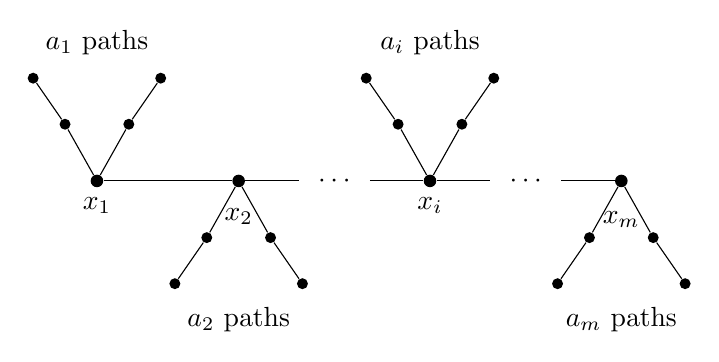
\begin{tikzpicture}[
    scale=0.9,
    vertex/.style={circle, fill=black, inner sep=1.6pt},
    smallvertex/.style={circle, fill=black, inner sep=1.4pt},
    labelnode/.style={rectangle, fill=none, inner sep=1pt}
]

% core vertices
\node[vertex, label=below:\(x_1\)] (x1) at (0,0) {};
\node[vertex] (x2) at (2,0) {};
\node[labelnode] at (2,-0.5) {\(x_2\)};
\node[labelnode] at (3.35,0) {\(\cdots\)};
\node[vertex, label=below:\(x_i\)] (xi) at (4.7,0) {};
\node[labelnode] at (6.05,0) {\(\cdots\)};
\node[vertex] (xm) at (7.4,0) {};
\node[labelnode] at (7.4,-0.55) {\(x_m\)};

% core path
\draw (x1)--(x2);
\draw (x2)--(2.85,0);
\draw (3.85,0)--(xi);
\draw (xi)--(5.55,0);
\draw (6.55,0)--(xm);

% arms at x1
\node[smallvertex] (x1a1) at (-0.45,0.8) {};
\node[smallvertex] (x1b1) at (-0.9,1.45) {};
\node[smallvertex] (x1a2) at (0.45,0.8) {};
\node[smallvertex] (x1b2) at (0.9,1.45) {};
\draw (x1)--(x1a1)--(x1b1);
\draw (x1)--(x1a2)--(x1b2);
\node[labelnode] at (0,1.95) {\(a_1\) paths};

% arms at x2
\node[smallvertex] (x2a1) at (1.55,-0.8) {};
\node[smallvertex] (x2b1) at (1.1,-1.45) {};
\node[smallvertex] (x2a2) at (2.45,-0.8) {};
\node[smallvertex] (x2b2) at (2.9,-1.45) {};
\draw (x2)--(x2a1)--(x2b1);
\draw (x2)--(x2a2)--(x2b2);
\node[labelnode] at (2,-1.95) {\(a_2\) paths};

% arms at xi
\node[smallvertex] (xia1) at (4.25,0.8) {};
\node[smallvertex] (xib1) at (3.8,1.45) {};
\node[smallvertex] (xia2) at (5.15,0.8) {};
\node[smallvertex] (xib2) at (5.6,1.45) {};
\draw (xi)--(xia1)--(xib1);
\draw (xi)--(xia2)--(xib2);
\node[labelnode] at (4.7,1.95) {\(a_i\) paths};

% arms at xm
\node[smallvertex] (xma1) at (6.95,-0.8) {};
\node[smallvertex] (xmb1) at (6.5,-1.45) {};
\node[smallvertex] (xma2) at (7.85,-0.8) {};
\node[smallvertex] (xmb2) at (8.3,-1.45) {};
\draw (xm)--(xma1)--(xmb1);
\draw (xm)--(xma2)--(xmb2);
\node[labelnode] at (7.4,-1.95) {\(a_m\) paths};

\end{tikzpicture}

\end{document}